\chapter{System Design and Methodology}
\label{chap5}

This chapter describes how the components introduced in Chapters~\ref{chap3}
and~\ref{chap4} are assembled into a working system and how the experimental
evaluation is structured. The theoretical background for the transformer
architecture, semantic embeddings, vector retrieval, and the evaluation metrics
was established in Chapter~\ref{chap3}, and the tools used to implement them were
described in Chapter~\ref{chap4}. This chapter focuses on the specific design
decisions made when connecting those components: the chunking strategies and their
parameters, the retrieval architecture, the prompt design, and the evaluation
protocol. The interactive application and the conversational memory strategies it
exposes are presented separately in Chapter~\ref{chap_app}.

\section{System Architecture Overview}

The system follows a retrieve-then-generate pipeline with conversational memory. A
user submits a question through the web interface. If the conversation has prior turns,
the question is first reformulated into a standalone query that can be understood
without the history. The reformulated query is sent to the retrieval layer, which
fetches the most relevant contract passages from the vector database using a
combination of dense semantic search and BM25 keyword matching. The retrieved
passages, the conversation history, and the original question are passed as context to
the language model, which generates a grounded answer. The answer is returned to the
user and stored in memory for the next turn.

The pipeline runs entirely locally. Both language models run on the host GPU with
4-bit NF4 quantization. The vector databases, the embedding model, and the BM25
index all operate on the same machine without external API calls. Langfuse Cloud
records per-request retrieval and generation latency and token counts for each query
issued during the evaluation.

\section{Document Indexing Pipeline}

This section describes how the contract corpus is prepared for retrieval: how the raw contract files are loaded, how they are split into passages under each of the three chunking strategies, and how the resulting chunks are embedded and stored in the vector databases.

\subsection{Contract Loading}

The 510 CUAD contracts are stored as plain text files. They are loaded using
LangChain's directory loader, which reads all text files from the data directory into
document objects that carry the source file path as metadata. This path is used later
by the retrieval layer to filter results to a specific contract when the user names one.

\subsection{Chunking Strategies}

Full contracts can run to hundreds of pages, but language models have fixed context windows, so each document is divided into smaller passages before indexing. Chunk size is a tradeoff: long chunks carry more context but dilute the relevant signal with surrounding text, while short chunks are precise but may split a clause across two segments and lose its meaning. Three strategies were implemented and compared, each applied to the full contract corpus.

\textbf{Fixed-size chunking} first splits the text at paragraph boundaries (double-newline separators), then groups adjacent paragraphs into chunks of up to 1,000 characters with a 200-character overlap between consecutive chunks. The overlap ensures that text near a boundary appears in both adjacent segments, reducing the chance that a relevant clause is cut in half. Because every split point is a paragraph break, a chunk edge does not fall in the middle of a sentence, so the limitation of the method is size control rather than boundary quality. It is fast to compute, but since it uses only this single separator, a paragraph that already exceeds 1,000 characters is kept whole rather than divided further. About a fifth of the chunks in the fixed collection are therefore larger than the target, the largest reaching nearly ten thousand characters, and these oversized chunks combine several clauses, which dilutes the relevant text when they are retrieved.


\textbf{Recursive character chunking} uses the same 1{,}000-character target and 200-character overlap, but tries to cut at natural boundaries before resorting to arbitrary splits: it attempts paragraph breaks first, then single newlines, then spaces, and only splits mid-text when a segment still exceeds the target size. Because a long paragraph is divided at the finest available boundary rather than kept whole, recursive chunking keeps every chunk close to the target size, whereas fixed-size splitting leaves long paragraphs as single oversized chunks.

\textbf{Semantic chunking} does not use a fixed size target. The embedding model computes the similarity between each pair of adjacent sentences, and a chunk boundary is placed wherever this similarity drops sharply, indicating a topic shift. The resulting chunks group sentences that discuss the same subject, so chunk sizes vary with the content of each contract section. This requires embedding every sentence before indexing, which makes it slower than the other two methods, but it can produce cleaner boundaries in legal text where topically related clauses are separated by formulaic boilerplate. The implementation uses LangChain's \texttt{SemanticChunker} with the default percentile breakpoint method: a boundary is placed wherever the cosine distance between two adjacent sentence embeddings exceeds the 95th percentile of all such distances measured within the document.


\subsection{Vector Database Construction}

After chunking, each collection is embedded with the all-MiniLM-L6-v2 model and
stored in a separate ChromaDB database. The three databases are built once and
persisted to disk. During all subsequent retrieval, they are loaded directly without
re-embedding. Each database functions as an independent index, so switching the
chunking strategy changes only which database is queried, with no other modification
to the pipeline.

\section{Retrieval Architecture}

This section describes how the system selects the passages passed to the language model. Retrieval combines dense semantic search with BM25 keyword matching, adds contract-specific routing so that each query is scoped to the named contract, and reformulates follow-up questions before searching.

\subsection{Dense Semantic Search}
The dense side of retrieval queries the ChromaDB index built for the active chunking strategy. The retrieval query, stripped of the CUAD boilerplate, is embedded with the same all-MiniLM-L6-v2 model used at indexing time, and the index returns the chunks whose embeddings are closest to the query in cosine similarity.

Because every question is scoped to a single named contract, the search is run over a large candidate pool and then filtered to that contract. For each query the index returns a pool of $k \times 10$ chunks, which are filtered to the chunks whose source path matches the named contract. The pool has to be large because the filter discards everything belonging to the other 509 contracts, and a smaller pool would frequently leave too few chunks from the target contract to fill the retrieval budget. With $k = 10$, 100 candidates are scored before filtering. The number of retrieved chunks $k$ is configurable from the Streamlit interface, and $k = 10$ was used for all six configurations in the automated evaluation. The value was chosen to balance retrieval recall against generation cost. A smaller $k$ risks excluding the relevant clause, especially given the vocabulary gap between the standardised CUAD category names and the wording used in the contracts, whereas a larger $k$ lengthens the input, raising generation latency and exposing the model to long-context degradation.

Scoping the search to one contract also removes the main reason a diversity-aware reranker would otherwise be needed. A single contract repeats boilerplate definitions and recurring cross-references, so a plain similarity search can return several near-duplicate passages. The contract-scoped pool combined with the keyword retriever described next, and the deduplication applied when the two result lists are merged, spread the final selection across different parts of the contract rather than returning repeated copies of the single strongest match.


\subsection{BM25 Keyword Retrieval and Hybrid Merging}

As discussed in Chapter~\ref{chap4}, semantic search alone fails when the query and the contract text use legally equivalent but semantically distant phrasing. A BM25 keyword index is built from the same document collection as the vector database and runs alongside the semantic retriever on every query. Running it unconditionally ensures the keyword bridge fires even when semantic search already returned enough passages, since the relevant clause may be worded too differently from the category name for the embedding model to rank it highly. To extend BM25 further, each CUAD category name is paired with a set of legal synonyms. When the query contains a recognised category, the BM25 query is expanded with the corresponding terms before retrieval. For example, a query for \textit{Expiration Date} is expanded with terms such as \textit{terminate}, \textit{termination}, \textit{expire}, \textit{notice period}, and \textit{duration}. This bridges the vocabulary gap between the standardised CUAD label and how the corresponding clause is actually written in practice. The semantic retriever keeps the clean category-and-details query so that embeddings are not diluted by the extra terms.

Results from both retrievers are merged into a single list by interleaving, with
duplicates removed, and trimmed to the target of 10 passages.

\subsection{Contract-Specific Retrieval}

CUAD evaluation questions always refer to a specific named contract. The system detects the contract name from the question, either from a quoted filename or from a human-readable title enclosed in quotes, and filters the semantic search results to passages whose source path matches that contract. A BM25 index is then built over that contract's passages alone and queried with the synonym-expanded query, so both retrievers contribute on every contract-scoped question rather than BM25 acting only as a fallback.


For clause categories that always appear near the top of a contract, such as the document title, the names of the parties, and the agreement date, vector search is bypassed entirely. The first few passages of the matching file are read directly from disk. Vector search is unreliable for these categories because the relevant text typically consists of proper nouns and formatting rather than semantically meaningful prose.

\subsection{Query Reformulation}

Before retrieval, CUAD's fixed boilerplate, \textit{``Highlight the parts (if any)
of this contract related to `[Category]' that should be reviewed by a lawyer. Details:
[description]''}, is stripped from the question. The retrieval query is reduced to
the clause category name and the details description only, giving the vector store a
cleaner signal. The stripped query is used for semantic search; for BM25, the same
query is additionally expanded with the category synonyms.

\section{Conversational RAG Chain}

This section describes the chain that ties retrieval and generation together for multi-turn use: how a follow-up question is condensed into a standalone query before retrieval, and the prompt that instructs the model to answer extractively from the retrieved excerpts.

\subsection{Question Condensation}

Follow-up questions in a conversation often contain unresolved references to earlier
turns, for example \textit{``What about the termination conditions?''} asked after a
question about a different clause. The retriever has no memory, so such references
must be resolved before retrieval. At the start of each turn where prior history
exists, the language model is prompted to rewrite the current question as a
self-contained query using the conversation history. The condensation prompt is shown
in Figure~\ref{fig:condense_prompt}.

\begin{figure}[h!]
    \centering
    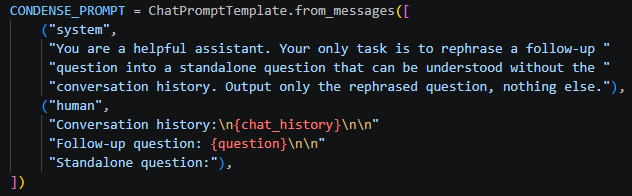
\includegraphics[width=0.84\linewidth]{figures/condense_prompt.png}
    \caption{Question condensation prompt used to resolve follow-up references before retrieval.}
    \label{fig:condense_prompt}
\end{figure}

\subsection{Question Answering Prompt}

The main prompt instructs the model to act as a legal assistant performing extractive question answering. It specifies that each retrieved excerpt is labelled with its source filename, and that if the question names a specific contract, only excerpts from that contract may be used. The prompt defines how to interpret CUAD-style category questions and gives explicit rules for categories such as \textit{Document Name}, \textit{Parties}, and \textit{Governing Law}. It also tells the model when to decline: a fixed not-found phrase must be used when the retrieved excerpts contain no clause related to the requested category, but if a related clause is present without the exact value asked for (a date, an amount, a duration), the clause itself must be quoted rather than refused. Using a fixed phrase rather than free-form refusal makes it straightforward to detect unanswerable responses programmatically during evaluation. Two further rules constrain answer style: the model is told to commit to the single most relevant quote rather than list possibilities with hedging language, and to quote only the minimal span that answers the question rather than reproduce the whole excerpt. The full system message is shown in Figure~\ref{fig:qa_prompt}.

%Both rules target failure modes observed in earlier runs, where correct answers were scored as refusals because of evasive phrasing, or as non-concise because the model included surrounding boilerplate. The full system message is shown in Figure~\ref{fig:qa_prompt}.


\begin{figure}[h!]
    \centering
    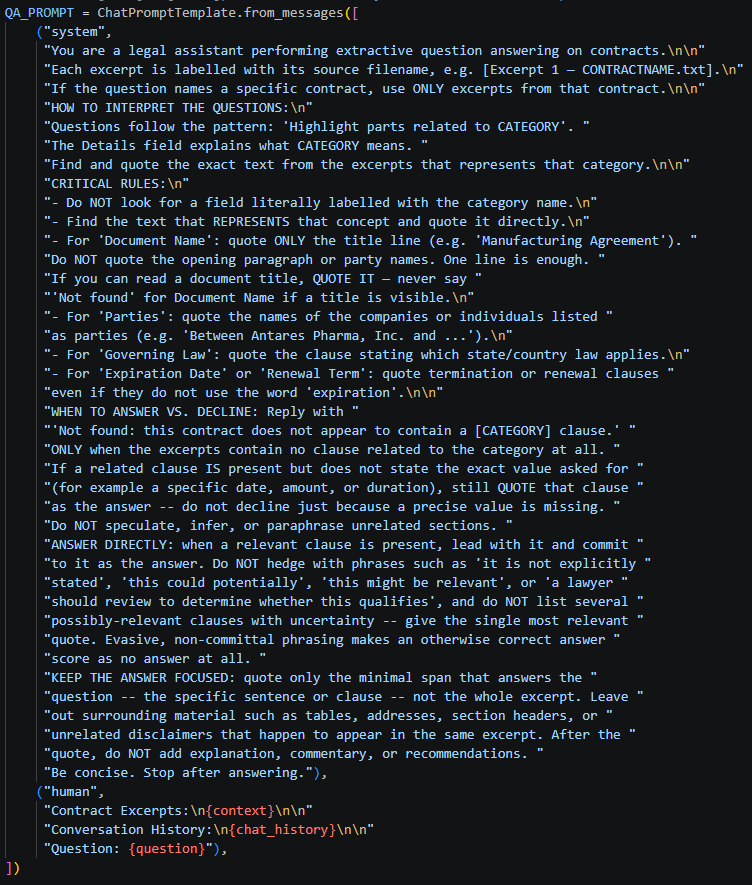
\includegraphics[width=\linewidth]{figures/qa_prompt2.png}
    \caption{Question answering prompt used in all six experimental configurations.}
    \label{fig:qa_prompt}
\end{figure}

\section{Experimental Configurations}

The three chunking strategies and two language models produce six configurations evaluated in the automated experiment. All six are run on the same question set under identical retrieval and prompt conditions. Table~\ref{tab:configs} lists the configurations. Conversation memory is deliberately excluded from this cross: because the automated evaluation resets the conversation history before each question, the windowed and summary strategies produce identical outputs in this
setting and would add no information to the quantitative comparison. They are instead evaluated separately, through a manual multi-turn test in the interactive application, in Chapter~\ref{chap_app}.


\begin{table}[h!]
\centering
\begin{tabular}{cll}
\hline
\textbf{Config} & \textbf{Chunking Strategy} & \textbf{Language Model} \\
\hline
1 & Fixed     & Llama 3.1 8B \\
2 & Fixed     & Mistral 7B   \\
3 & Recursive & Llama 3.1 8B \\
4 & Recursive & Mistral 7B   \\
5 & Semantic  & Llama 3.1 8B \\
6 & Semantic  & Mistral 7B   \\
\hline
\end{tabular}
\caption{The six experimental configurations evaluated in this thesis.}
\label{tab:configs}
\end{table}

\newpage
\section{Evaluation Methodology}

This section describes the protocol used to evaluate the six configurations: how the question sample is drawn, how RAGAS and the LLM-as-a-Judge produce their scores, and how the no-retrieval baseline is run for comparison.

\subsection{Question Sampling}
\label{sec:eval-sampling}

The evaluation uses the 20-question stratified sample described in Section~\ref{sec:question-sampling}. The same set is used for all six configurations and the
no-retrieval baseline, so all comparisons are made on identical inputs.


Before each question is submitted, the title of the corresponding contract is
prepended in the format \textit{``Contract Title'' question text}. This triggers
the contract-specific retrieval and prevents the pipeline from searching across all 510 contracts for each query.

\subsection{RAGAS Evaluation}

For each configuration, the system's answers and retrieved context are passed to the RAGAS evaluator. RAGAS requires an external language model to make the judgements for Faithfulness, Answer Relevancy, Context Precision, and Context Recall. The evaluator used in this thesis is OpenAI's GPT-4o-mini, accessed through the OpenAI API. GPT-4o-mini was chosen because it consistently produces well-formed JSON verdicts for the structured scoring tasks RAGAS requires, at a cost low enough to evaluate the full six-configuration sweep without budget concerns. Any scores returned as null are excluded from the configuration averages.

Unanswerable questions are excluded from RAGAS evaluation. When the ground truth is
empty, Context Recall is zero by definition regardless of what was retrieved, and
Faithfulness becomes ill-defined. Including these questions would suppress the
averages in a way that does not reflect retrieval quality.

\subsection{LLM-as-a-Judge Evaluation}

Correctness and conciseness are scored by the same external model used for RAGAS.
Correctness is evaluated only for answerable questions, comparing the system's answer
against the CUAD ground truth span on a 1--5 scale. Conciseness is evaluated for all
non-error answers regardless of whether the question is answerable. Both scores are
normalised to the $[0, 1]$ interval using the formula defined in
Chapter~\ref{chap3}. The judge receives the question, the ground truth (for
correctness), and the system's answer, and must respond with a JSON object containing
the score and a one-sentence justification. The correctness and conciseness scoring prompts are shown in Figures~\ref{fig:judge_correctness_prompt} and~\ref{fig:judge_conciseness_prompt}.

\begin{figure}[h!]
    \centering
    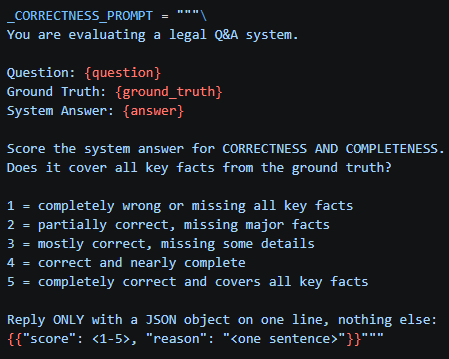
\includegraphics[width=0.6\linewidth]{figures/judge_correctness_prompt.png}
    \caption{LLM-as-a-Judge correctness prompt.}
    \label{fig:judge_correctness_prompt}
\end{figure}

\begin{figure}[h!]
    \centering
    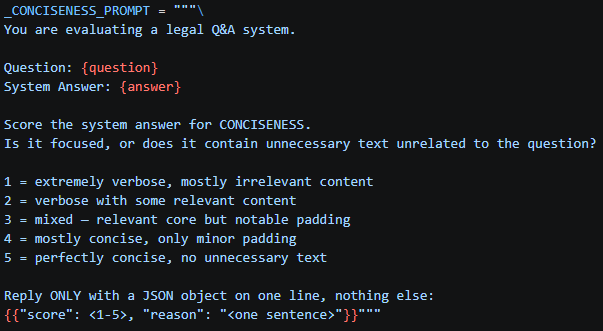
\includegraphics[width=0.8\linewidth]{figures/judge_conciseness_prompt.png}
    \caption{LLM-as-a-Judge conciseness prompt.}
    \label{fig:judge_conciseness_prompt}
\end{figure}

\newpage
\subsection{No-Retrieval Baseline}

To measure the contribution of retrieval, each language model is also run without any retrieved context on the same twenty questions. The model receives only the question and a brief instruction to answer from general legal knowledge or to respond with \textit{``Not found''} if the answer requires reading the specific contract. Since there is no retrieved context, RAGAS metrics are not applicable to the baseline. Correctness and conciseness are scored by LLM-as-a-Judge, allowing a direct comparison of judge correctness between the RAG configurations and the no-retrieval baseline for each language model. This comparison quantifies how much retrieval contributes to answer quality over what the model already knows from training. The baseline prompt is shown in Figure~\ref{fig:baseline_prompt}.

\begin{figure}[h!]
    \centering
    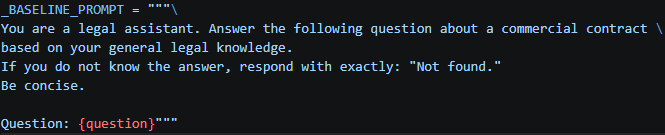
\includegraphics[width=0.88\linewidth]{figures/baseline_prompt.png}
    \caption{No-retrieval baseline prompt.}
    \label{fig:baseline_prompt}
\end{figure}

